The results from running the Jacobi rotation algorithm will vary with how 
$n_{\mathrm{step}}$ and $\rho_{max}$ are chosen. First of all, it would be useful to find
out how large the matrix needs to be for the algorithm to produce the first few
eigenvalues with four leading digits. At that point, the precision is high
enough for our purposes. Second, we'd like to see how the precision in the
eigenvalues depend on the choice of $\rho_{max}$. 

By doing more of a guess than calculation, we set $\rho_{max} = 5$. The
algorithm is then used to find the eigenvalues of matrices with increasing
dimensions. The range for $n_{\mathrm{step}}$ is narrowed down to $n_{\mathrm{step}} \in 
[150,300]$ to see the relative difference more clearly. Figure \refig{nreldiff} shows 
the result. 
%
\begin{figure}[htpb]
\centering
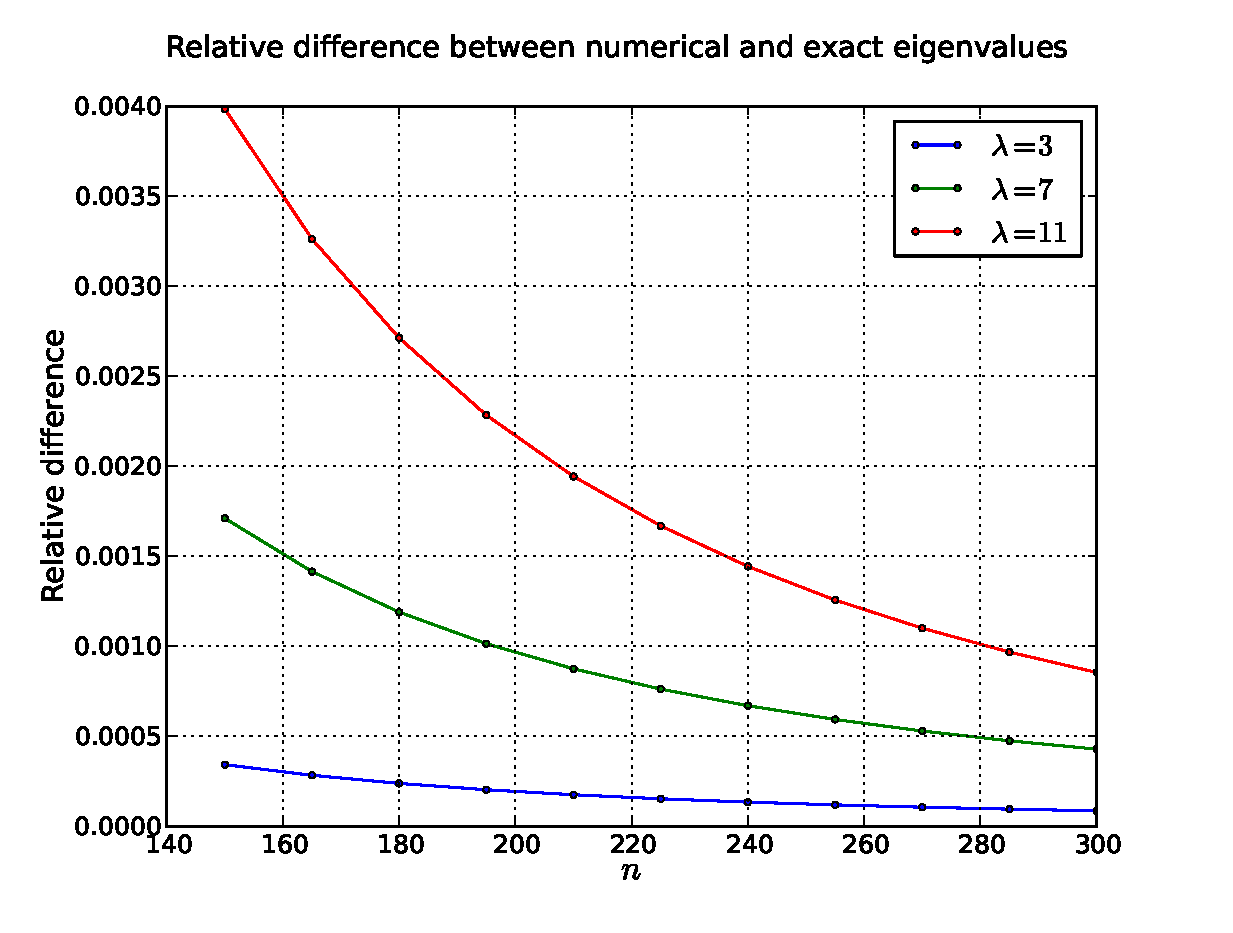
\includegraphics[width=1.0\textwidth]{images/nreldiff2.eps}
\caption{The figure shows how much the numerical eigenvalues differ from the analytical
	ones as $n_{\mathrm{step}}$ increases. Here we have $\rho_{max} = 5$.}
\label{fig:nreldiff}
\end{figure}
%
It's obvious that $\lambda_0 = 3$ varies the least, and has four correct leading digits
throughout the plot. The second eigenvalue $\lambda_1 = 7$ varies more, and settles
at four correct leading digits for about $n_{\mathrm{step}} = 210$. The third eigenvalue,
$\lambda_2 = 11$, has four correct leading digits for all $n_{\mathrm{step}}$ that are shown in 
\refig{nreldiff}. This means that when $n_{\mathrm{step}} = 210$, all three eigenvalues show 
four correct leading digits. 

The precision of the eigenvalues will also depend on $\rho_{max}$. By doing the same
procedure as above, but keeping $n_{\mathrm{step}}$ constant and vary $\rho_{max}$ instead, we
get the result shown in figure \refig{rhoreldiff}.
%
\begin{figure}[htpb]
	\centering
	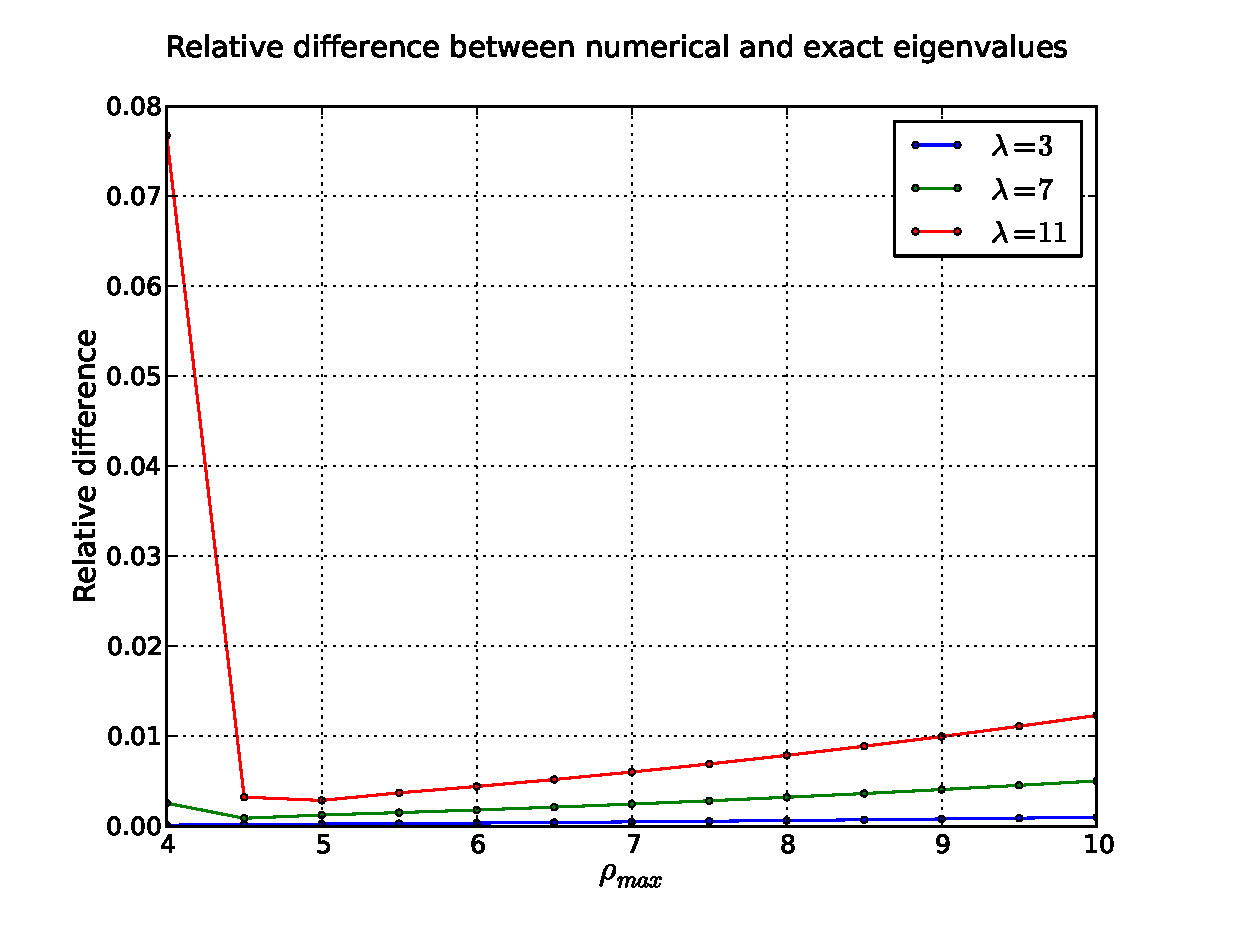
\includegraphics[width=1.0\textwidth]{images/reldiff2.eps}
	\caption{The figure shows how the numerical eigenvalues differ from the analytical
		ones as $\rho_{max}$ increases. Here we have $n_{\mathrm{step}} = 210$.}
	\label{fig:rhoreldiff}
\end{figure}
%
Again, the range of $\rho_{max}$ is narrowed down to $\rho_{max} \in [4,10]$ in order to
highlight the interesting part. For $\rho_{max} = 4$ both $\lambda_1$ and $\lambda_2$ are
below our precision limit. Already at the next step, $\rho_{max} = 4.5$, they both
reach four leading digit precision. This holds true for $\rho_{max} = 5$ as well, although
the graph grows. For higher values, the precision just lowers.
So far, we can conclude that $\rho_{max} = 4.5$ gives the greatest accuracy.

It can be useful to know how many transformations are needed before all non-diagonal
elements have become zero. Of course, this means that we need to define what we mean by
``zero''. In the algorithm, we set a threshold $\epsilon$ that restricts the value of the
max element on the non-diagonal. By setting this to a small value, for example $\epsilon =
10^{-8}$, we know that no off-diagonal element is above this limit. Any element below the
value of $\epsilon$ is then essentially zero.

Obviously, the number of transformations must be a function of $n_{\mathrm{step}}$. Larger
$n_{\mathrm{step}}$ means larger matrix, and more elements need to be transformed.
To estimate how many transformations are needed, we run the algorithm for several
$n_{\mathrm{step}}$ with $\rho_{max} = 4.5$. This gave us some number of transformations,
with the corresponding dimensionality of the matrix. These points were then imported into 
MATLAB, so we could approximate a polynomial with the given data. The number of transformations as function of $n_{\mathrm{step}}$ was approximated to a second-order polynomial
%
$$ T(n_{\mathrm{step}}) \approx 1.69 \cdot n_{\mathrm{step}}^2 - 3.76 \cdot n_{\mathrm{step}}
+ 10.16 $$
%
MATLAB also tells us that the approximation carries with it a root-mean square error
(RMSE) of 44.5, which means that the polynomial approximation has a relatively low
precision. By increasing the data resolution, one could achieve a better approximation.
As $n_{\mathrm{step}}$ grows large, the last constant term will hardly contribute, so we 
might as well exclude it. The first order term will also be quite small compared to
$n_{\mathrm{step}}^2$, so we will ommit that one as well, since we're only after a rough 
estimate of how the number of transformations vary with $n_{\mathrm{step}}$. This means that
$$ T(n_{\mathrm{step}}) \approx 1.69 \cdot n_{\mathrm{step}}^2 $$
where $T(n_{\mathrm{step}})$ represents the number of transformations, and $n_{\mathrm{step}}$
is the dimensionality of the matrix. 

There are other methods for finding eigenvalues of a general og symmetric matrix. In
addition to the Jacobi rotation algorithm, we have Householder's algorithm and Lanczos'
algorithm, to mention a few. We want to compare the runtime of our program to some
other program where we implement another eigenvalue solver. Armadillo has a function 
$\verb|eig_sym()|$ that takes a symmetric
matrix and returns its eigenvalues and eigenvectors. We will use this function to compare
with the Jacobi algorithm. 

The Armadillo function uses a standard eigen decomposition algorithm by default. One
can change this by giving $\verb|"dc"|$ as argument, and the function switches to a
divide-and-conquer algorithm. This provides slightly different results, but is notably
faster for large matrices. Table \reftab{runtime} shows the runtimes.
%
\begin{table}[htpb]
	\centering
	\begin{tabular}{|p{1cm}|p{1.5cm}|p{2cm}|p{2.5cm}|}
		\hline
		$n_{\mathrm{step}}$ & \textbf{JRA} & \textbf{Armadillo} & \textbf{Armadillo DC} \\
		\hline
		\hline
		\textbf{50} &  0.07 s & 0.00 s & 0.00 s \\
		\textbf{100} &  0.99 s & 0.00 s & 0.00 s \\
		\textbf{150} &  4.94 s & 0.01 s & 0.01 s \\
		\textbf{200} & 15.61 s & 0.02 s & 0.01 s \\
		\textbf{250} & 37.77 s & 0.03 s & 0.02 s \\
		\textbf{300} & 77.68 s & 0.05 s & 0.02 s \\
		\hline
	\end{tabular}
	\caption{The table shows the runtime for various algorithms with different matrix
	sizes.}
	\label{tab:runtime}
\end{table}
%
It is clear that the Armadillo function is superior to our implementation of the Jacobi
algorithm (JRA). In addition to being a lot faster, the Armadillo function it also returns
the eigenvectors. In our implementation of the Jacobi method, only the eigenvalues are
calculated.

Although it is much more efficient to use the Armadillo function, implementing the Jacobi
rotation algorithm gives us valuable insight in how some eigenvalue solvers work. It is
slow, especially for large matrices, but very easy to implement. For every transformation,
the previous elements which were set to zero, may have become different from zero. This
means that it needs to transform these elements again. That is one of the reasons for why 
the method is slow.

How does the relative
difference behave for various $n_{\mathrm{step}}$, compared to figure \refig{nreldiff}? 
%
\begin{figure}[htpb]
	\centering
	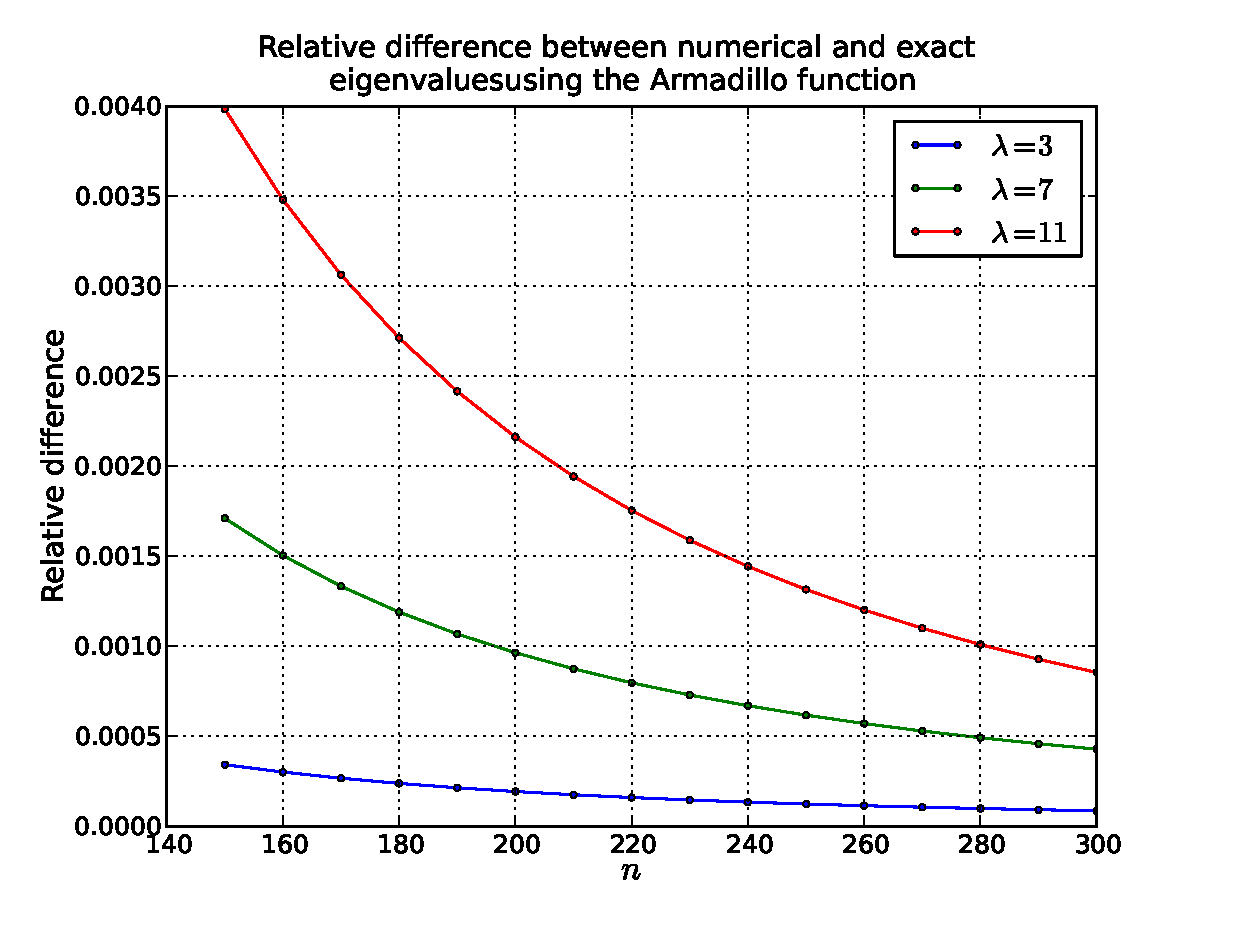
\includegraphics[width=1.0\textwidth]{images/armareldiff2.eps}
	\caption{The figure shows how the numerical eigenvalues differ from the analytical,
		using the Armadillo eigenvalue solver. Here $\rho_{max} = 5$.}
	\label{fig:armareldiff}
\end{figure}
%
Figure \refig{armareldiff} shows a similar result to figure \refig{nreldiff}. From this we
can conclude that the relative difference between numerical and analytical eigenvalues
from the Armadillo function, vary the same way as the Jacobi method. Not only is the
Armadillo function much faster, but it is also just as accurate as the Jacobi method.

